% !TeX root = main.tex
\chapter{Introduction \label{ch1-intro}}

Sensors fail. Failure rates often depend on the sensor as well as the complexity of the system into which the sensor is integrated. Historically, sensors (latin: \textit{sentire}: perceive) are defined as entities that measure physical conditions. This information then gets transmitted by signals that are emitted by the sensors \cite{din_din_1995, pena-consuegra_manufacturing_2023}. Aircraft sensors generally emit an electric current that gets transformed into a digital signal by an Analog to Digital Converter (ADC). This digital signal then flows through other stages until it reaches the Main Aircraft Bus where it can be used by the aircrafts systems.

Within this works scope the ISTAR aircraft (In-flight Systems & Technology Airborne Research) gets examined. The ISTAR is a Falcon 2000LX business jet that is equipped with various additional sensors including strain gauges, accelerometers and changing experimental configurations. öö-

\begin{figure}
    \centering
    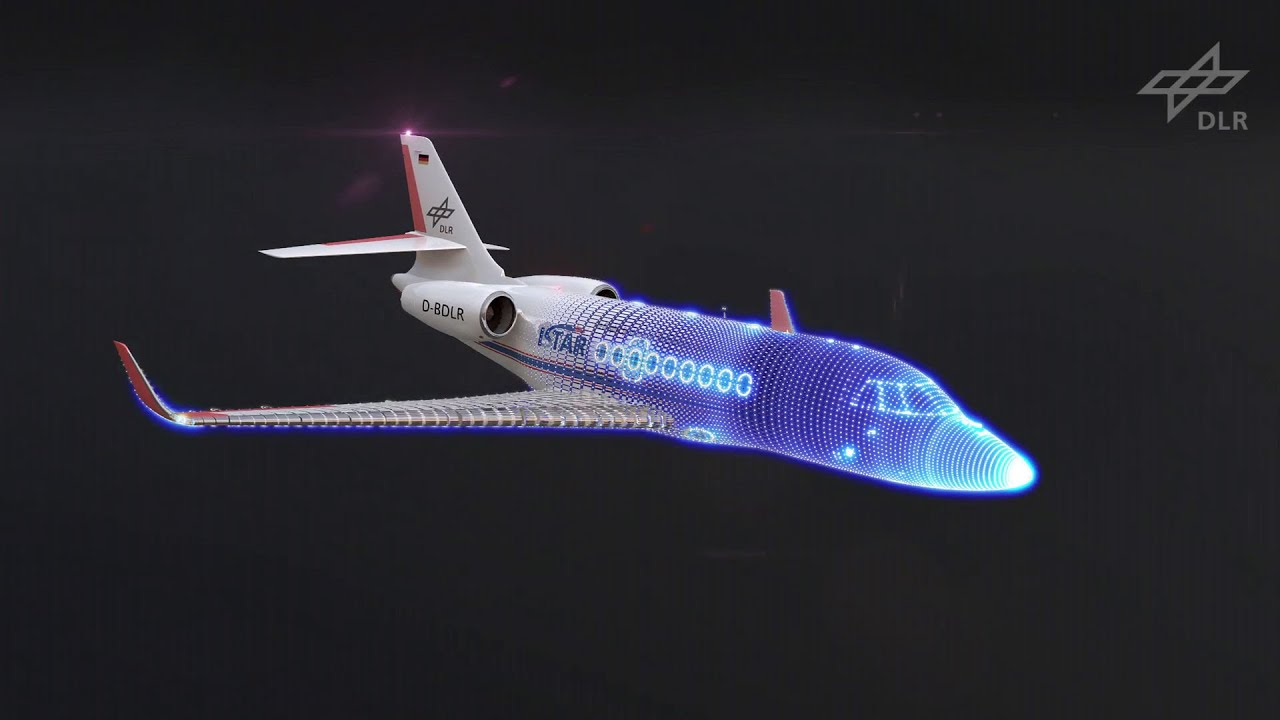
\includegraphics[width=0.7\textwidth]{istar_semitransparent}
    \caption{The ISTARs sensor data systems will be analysed within this work \cite{dlr_dlr-forschungsflugzeug_2020}}
    \label{fig:istar_semitransparent}
\end{figure}

\paragraph{What?}
%\section{What}
%Q:What is going to be examined within this thesis?
%E:

The ISTAR aircraft is currently the aircraft generating the most data for the DLR's research aircraft fleet at the Brunswick Research Site. This fleet is Europe's largest, consisting of 12 aircraft employed for research purposes ranging from atmospheric research to testing operating limits that are pushing the aircraft operating envelope.
The data acquisitioning system (DAQ) plays a focal role in the generated data since it is the central data hub within the airplane. Making the DAQ as well as the sensor data the central point of this work.
In conjunction with the FAIR principles this work also focuses on reusability of the components of this work as well as interoperability with outside algorithms. Allowing the results of this work to be accessible by uploading them to the FAIR skystash data-platform and making condensing errors into tags and using conventions to catalyze digitalization to make the resulting data findable.
Hence, making it the goal of this thesis to examine the ISTAR DAQ in detail to detect sensor behaviour anomalies and implement a clear infrastructure to fulfill FAIR principles.

\paragraph{Why?}
%Q: Why is this important?

It is then important to reduce manual overview of sensors. Currently, much manual postprocessing is needed to get an overview over the large datasets. Large datasets however are difficult to work with due to being too large for a single computer. Necessitating a server architecture for work with this size of data.
Another benefit of this work may be to reduce downtime of the Aircraft due to sensors. A diagnostic tool for detecting sensor behavior can facilitate the processes and allow a quicker follow up to detect sensor errors since currently system information is distributed and not clearly perceivable.

To achieve this it is vital to increase the fault detection rate since sensor faults are frequently not detected). Commonly, a sensor- or system-failure may not be detected during a flight experiment but weeks after. This rescheduling within the aircrafts full timetable makes it even more economically important to implement a system to catch sensor faults and failures to avoid the need for an experiment to be reflown. A worst case scenario could be that a whole experiment needs to be repeated with the configuration needing to be recustomized and refitted which is a time- and funding intensive task.
Additionally, it is important to increase reaction time. Often errors are detected weeks after the flight is over. With a software detecting errors directly after sensor data is extracted from the aircraft errors may be detected on the same day. allowing a quicker reaction maybe repeating the experiment during the affixed timeslot.

Safety critical errors may be detected earlier since the proposed routine has potential to go beyond the scope of commercially tested software that is generally employed within aircraft and generally rudimentary resulting from the desire to employ very stable software.
Once, a baseline routine is in place. It is then possible to build a foundation for a reliability index for sensors. This is vital for big data operations within digitalization and the skystash project. This should be able to implemented by plug and play into this works results. Allowing for quick implementation of custom data quality algorithms.

Another motivation for this work is the fulfillment of the FAIR (Findable, Accessible, Interoperable, Reusable) principles. FAIR principles are the new standard within the DLR for research data management. The use within operations however are far from the fulfillment. Documents containing descriptions of sensors and setups are distributed among multiple employees obstructing any efforts to comprehend the already complex aircraft system and its inherent generation of data.

The proposed work is then nothing short of essential, building a tool for detection and avoidance of sensor failures to mitigate risks associated with experimental setups since aircraft hours are expensive and the amount of sensors is vast.

\begin{figure}
    \centering
    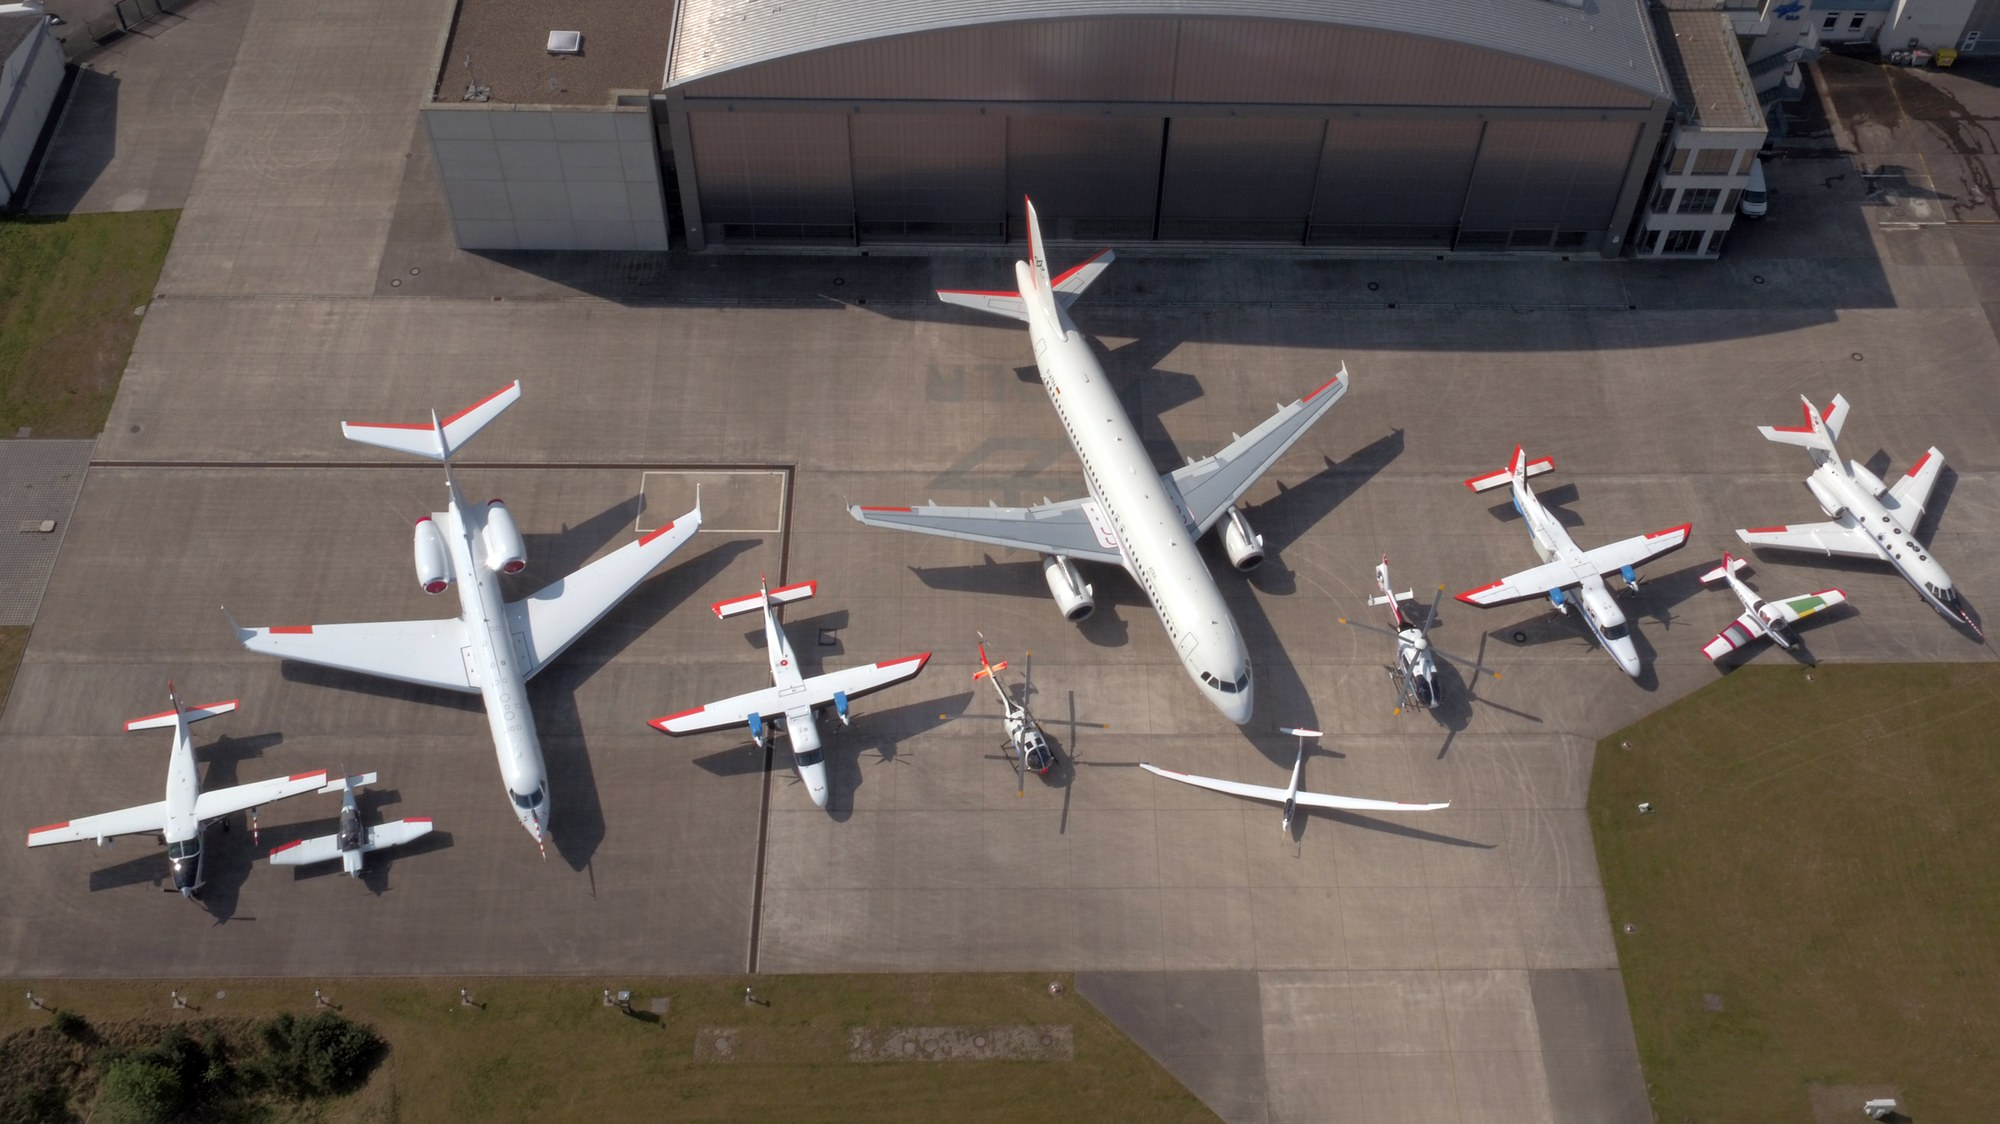
\includegraphics[width=0.7\textwidth]{dlr_fleet.jpeg}
    \caption{The DLRs research fleet \cite{dlr_dlr-fleet_2018}}
    \label{fig:dlr_fleet}
\end{figure}

\paragraph{Origin of Data}
%Q:Where does ISTAR data come from?
%E:-
The Flight Test Data by the ISTAR gets generated by a base DAQ system by IMC co. This base contains inputs from the main aircraft data bus, the experimental nose boom, experimental strain gauges and acc sensors as well as an experimental Inertial Measuring Unit (IMU) combined with a GNSS-System.
In addition, complementary DAQs are added to fulfill given experiment requirements.
In regard to system complexity it is notable that the main aircraft bus data originates from various sources, ranging from air data that gets measured by a sensor working on an electric current which then gets transformed by an Analog Digital Converter (ADC) into a digital, discretized signal which then gets fed into the main aircraft bus system. Such a signal would then getstransmitted to the IMC DAQ making troubleshooting a multifaceted problem within this system.

%C: Data originates from all over the aircraft and gets collected in the aircraft experimental DAQ.

%\section{Origin}

%Matthews flowchart(dataflow from sensor voltage through computer-computer-user)
%Exemplary for a single sensor.

\paragraph{How?}
%Q: How to solve this rather extensive problem of SHM?
To now solve this extensive problem of SHM, it is possible to employ one of many existing methods in the field of Fault Detection and Mode Analysis (FMEA).

FMEA is a common problem in engineering disciplines and everywhere where systems become complex. %Literature is rich in this regard, so finding an appropriate solution should be a feasible undertaking
This problem also gets facilitated by the work that is already happening within the digital twin program within the DLR. A data space is already in development and is supplied with Flight Test Data which aids this work.
It is then necessary to allow clear software interfaces to facilitate future extensions and modes to allow reaching a quick overview over sensor errors.
FMEA is a rich field in which much energy has already been invested into similar problems. A new challenge arises from the implementation into a dynamic digital system also keeping in mind to remain open for new changes and addons.

%Q: whats the context on this work?

\paragraph{Context}
This work happens within the DLRs effort to digitize and digitalize research data and update its research data management strategy.
%Part of DigECat project for ISTAR digital twin
Within this project's scope, the development of skystash architecture is advanced to beyond prototypical level, allowing upload and distribution of research data by using the skystash cloud.
Within the scope of future work lies the expansion of metadata management on a larger scale, metadata frameworks already exists but challenges arise from indexing and providing a digital replica of long paper trails. Aircraft are highly complex systems that amass a great amount of paperwork since even its tiniest screws require a highly documented certification process.
%Further big data efforts also include data analytics allowing for easy scaling of this data base format
%For now, present work: work on prototypes of metadata management to represent sensor data. Calculations then can happen based on datasets with provided metadata without additional inputs.

Digitalization and the digital twin are the inherent adjuncts of this work. A database with data already exists. now it is time to structure metadata allowing for this work to happen dynamically. Building upon this, further metadata may be fed into the system allowing further analytics to be developed.


\paragraph{Summary}

This work will examine the sensor data of the ISTAR aircraft, examining various algorithms and methods for FMEA. Then developing a software that allows dynamic implementations of various FMEAs to generate a dynamic backend facilitating development and finally generating reports on data quality for the aircraft systems. FAIR principles are vital for future legibility and exchangeability of data and hence become a central part of this thesis facilitating future use of the results generated within this work.